% Indicate the main file. Must go at the beginning of the file.
% !TEX root = ../main.tex

%%%%%%%%%%%%%%%%%%%%%%%%%%%%%%%%%%%%%%%%%%%%%%%%%%%%%%%%%%%%%%%%%%%%%%%%%%%%%%%%
% 03_results
%%%%%%%%%%%%%%%%%%%%%%%%%%%%%%%%%%%%%%%%%%%%%%%%%%%%%%%%%%%%%%%%%%%%%%%%%%%%%%%%


\section{Results}
\label{section3}

\subsection{Hyperparameter Tuning}

Table \ref{tab:hyperparameters_results}

\begin{figure}[h!]
    \centering
    \captionsetup{width=.7\linewidth}
    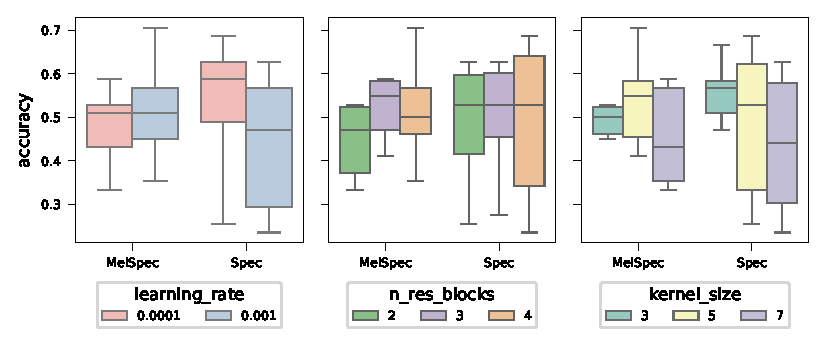
\includegraphics[width=0.85\textwidth]{figures/hyperparameters_boxplot.pdf}
    \caption{Accuracy of the models for different hyperparameter grouped by the transformation type.}
    \label{fig:hyperparameters_boxplot}
\end{figure}

\begin{figure}[h!]
    \centering
    \captionsetup{width=.7\linewidth}
    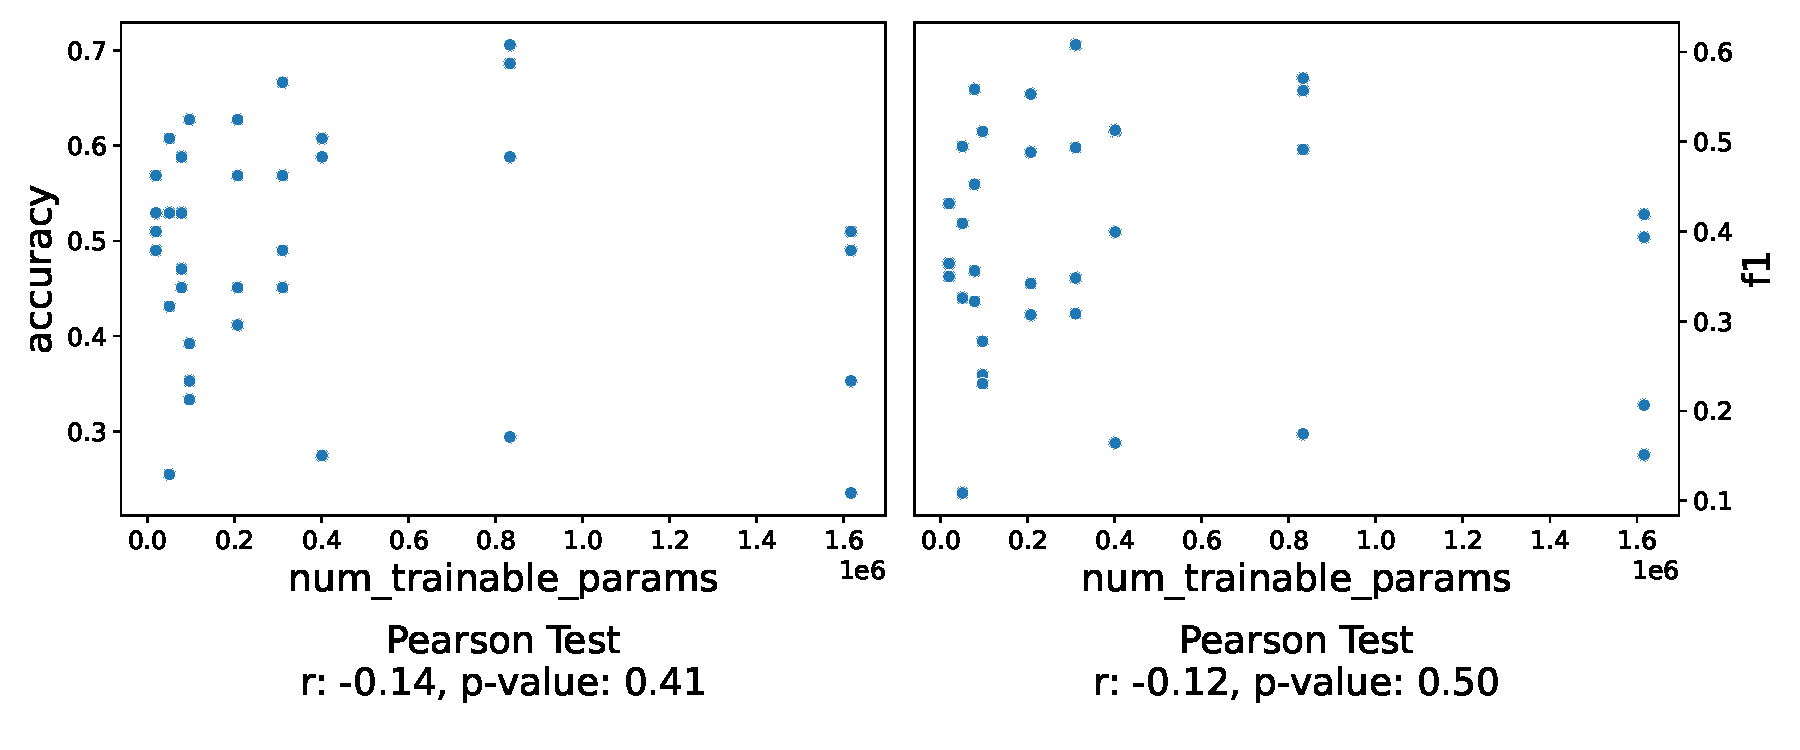
\includegraphics[width=0.85\textwidth]{figures/hyperparameters_scatterplot.pdf}
    \caption{Model size compared to the accuracy and F1 Score of the models.}
    \label{fig:hyperparameters_scatterplot}
\end{figure}

\begin{figure}[h!]
    \centering
    \captionsetup{width=.7\linewidth}
    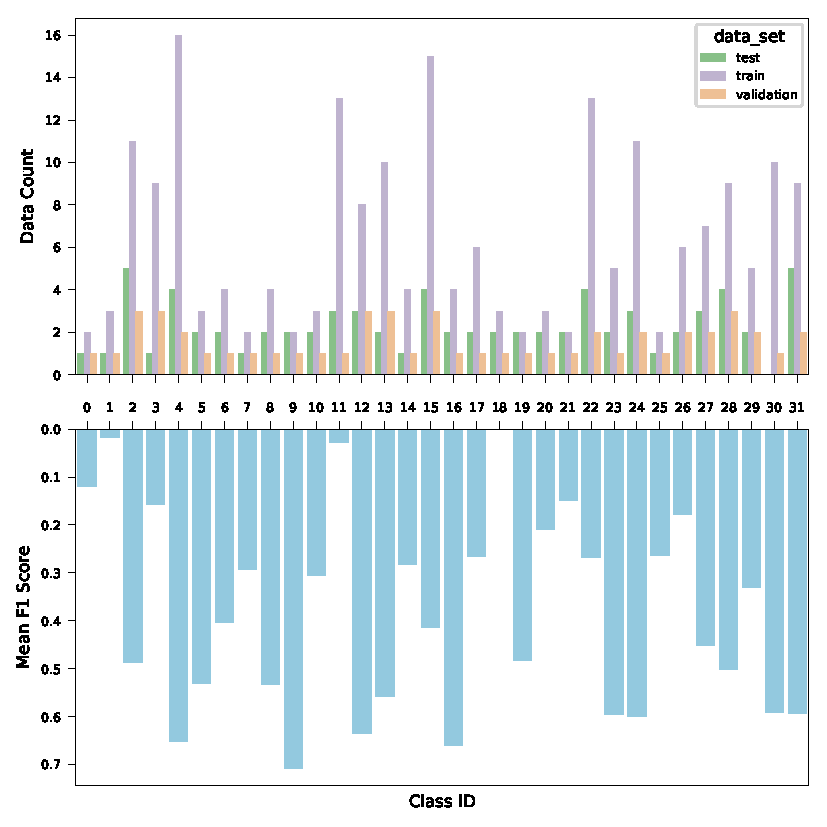
\includegraphics[width=0.85\textwidth]{figures/f1_per_class.pdf}
    \caption{F1 Score per class as mean trough all models compared to data distribution.}
    \label{fig:f1_per_class}
\end{figure}



\subsection{Performance of the best Model}

The best performing configuration for the model was found to be the one with the following hyperparameters:

\begin{itemize}
    \item \textbf{n\_mels:} 64
    \item \textbf{n\_res\_blocks:} 4
    \item \textbf{learning\_rate:} 0.001
    \item \textbf{kernel\_size:} 5
\end{itemize}

On the test set, the model achieved an accuracy of 0.649. 
The confusion matrix for the test set is shown in Figure \ref{fig:confusion_matrix_best}.

\begin{figure}[h!]
    \centering
    \captionsetup{width=.7\linewidth}
    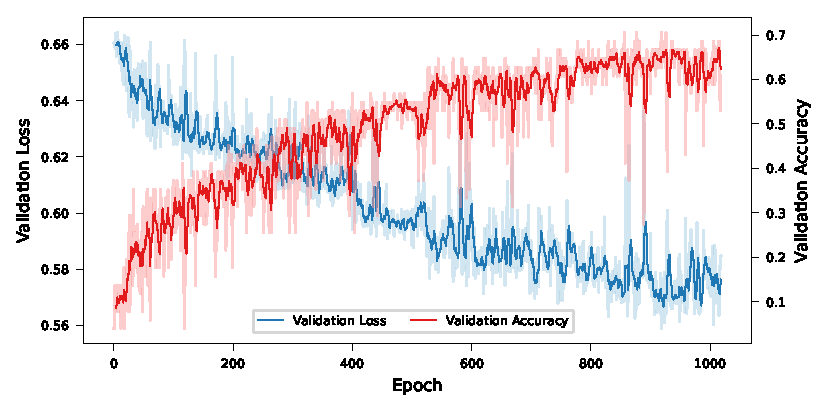
\includegraphics[width=0.85\textwidth]{figures/loss_acc_best.pdf}
    \caption{
        The validation loss and accuracy of the best model. Light version is not smoothed 
        and dark version is smoothed with a window size of 5.}
    \label{fig:loss_acc_best}
\end{figure}


\begin{figure}[h!]
    \centering
    \captionsetup{width=.7\linewidth}
    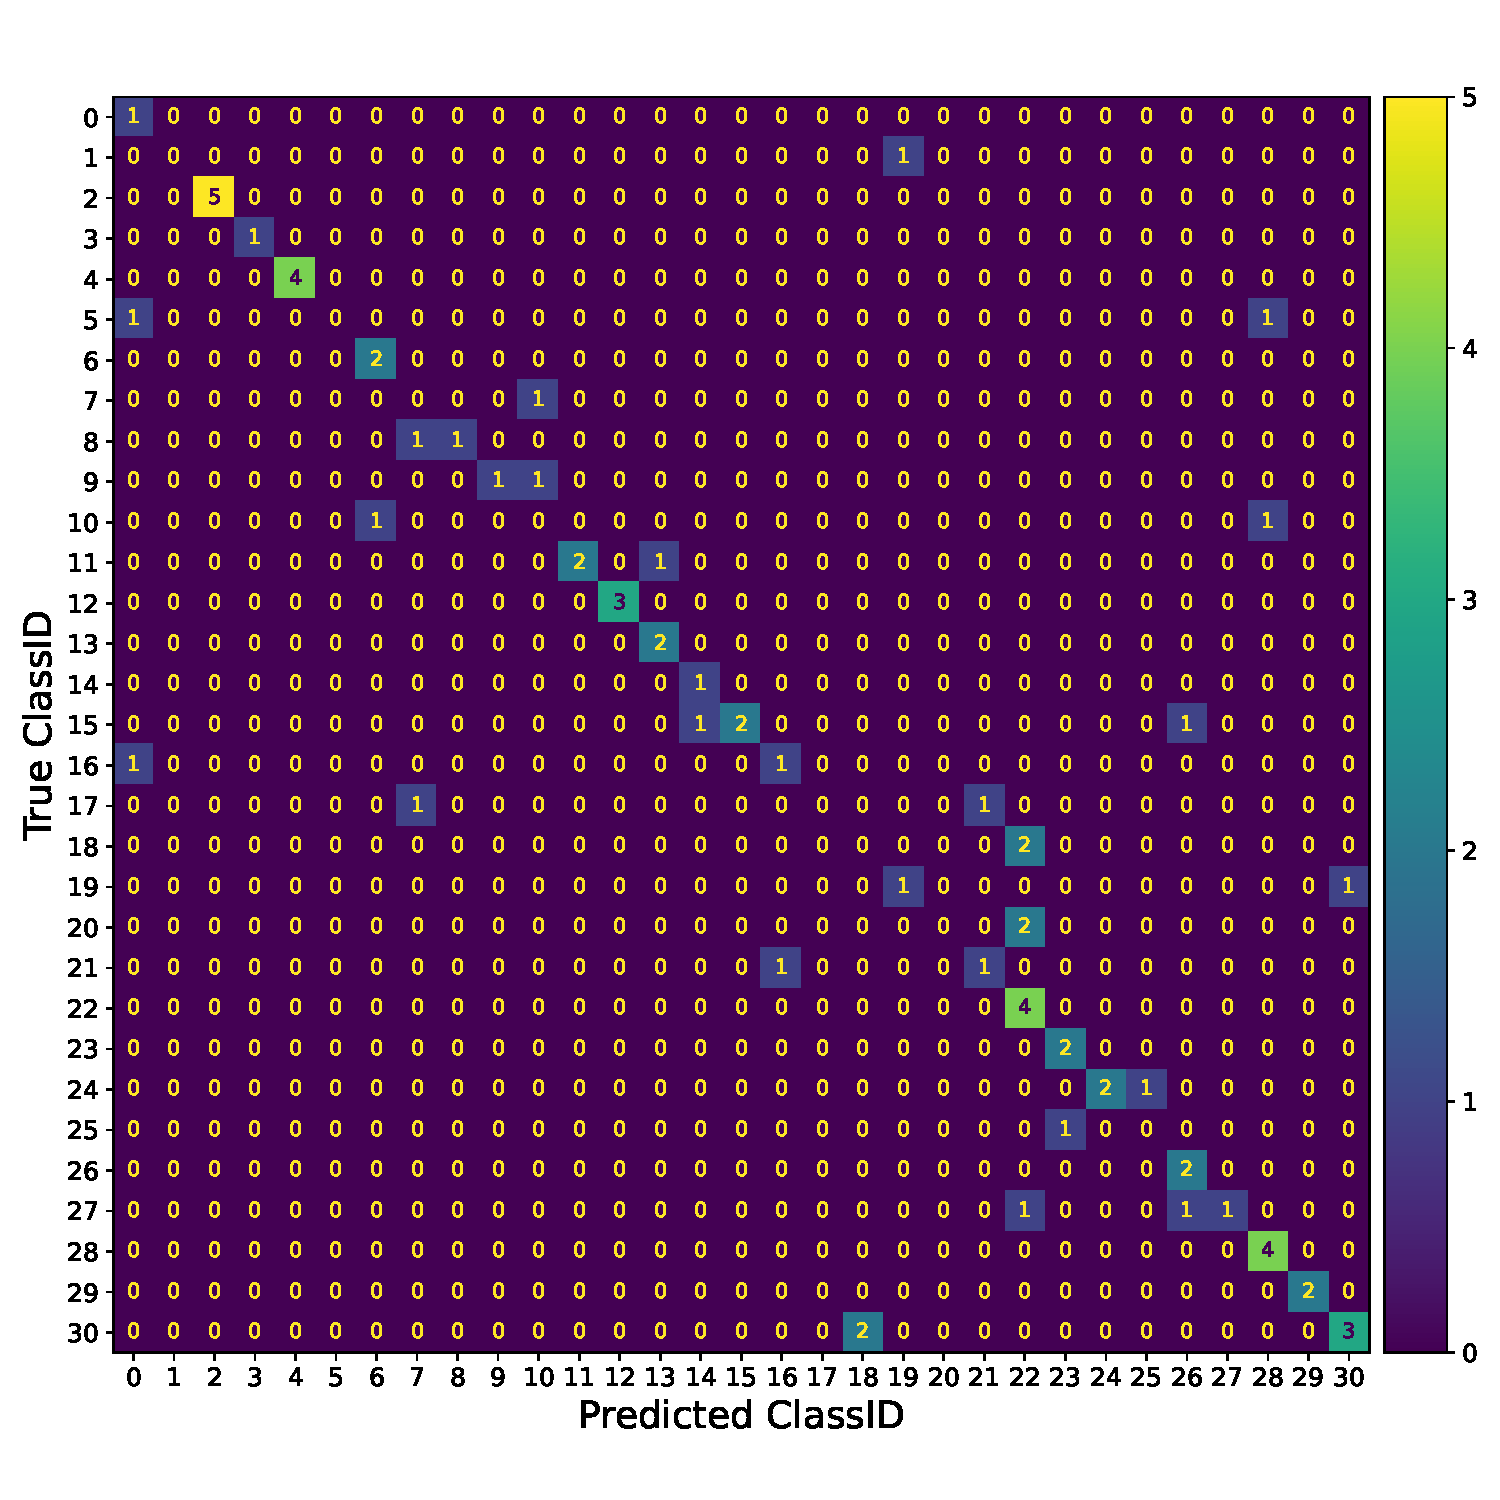
\includegraphics[width=0.85\textwidth]{figures/confusion_matrix_best.pdf}
    \caption{Confusion matrix for the predictions of the test set using the best model.}
    \label{fig:confusion_matrix_best}
\end{figure}